%!TEX root = ../thesis.tex
%*******************************************************************************
%*********************************** First Chapter *****************************
%*******************************************************************************

\chapter{Correlations of the impedance plethysmography device}  %Title of the First Chapter
\label{chapter correlations}
\ifpdf
    \graphicspath{{Chapter6/Figs/Raster/}{Chapter6/Figs/PDF/}{Chapter6/Figs/}}
\else
    \graphicspath{{Chapter6/Figs/Vector/}{Chapter6/Figs/}}
\fi

The previous chapter \ref{chapter results} showed the performance of the designed impedance plethysmography device and the data collected in resistivity value and its equivalent in blood flow. It was shown the capability of the instrument on detecting changes during three different kinds of occlusion. Furthermore, it was presented the data collected from the other devices such as Doppler ultrasound, LDF, PPG and ECG. 

In this chapter, the correlation between the different measurements gathered will be analysed. The aim of this correlational investigation is understanding what the contributing factors towards the impedance plethysmography signal are. As it has been explained in previous chapters, the change of the volume in the forearm section let to estimate the blood flow from the segment. However, both arterial and venous blood contributes to the information of blood flow calculated by the iPG device. It is not clear, how much of the blood flow belongs to any of the types of blood. Besides, it was shown that main blood vessels contribute to the measurement of blood flow but microcirculation might also provide additional information under the iPG waveform. 

\mynote{This paragraph is quite an statement. I have to verify if I can really calculate how much is the contribution of the micro circulation and the other types of blood flow.}

%********************************** %First Section  **************************************
\section{Analysis of the the heart beat detection in the frequency domain} %Section - 6.1
\label{section correlation 1} 
The signals obtained from all the devices during the experiment are synchronous to the heart beat. This synchronisation reflects that in their dynamic component the systolic peak is also present in the waveform of these instruments.

Nonetheless, some noises impact negatively to the proper detection of the systolic peaks during the study. The algorithm designed can detect the shape of the waveform by finding the foot of the signal and its peaks. Nevertheless, some of the peaks might be missing because of the noise levels.

A Fast Fourier Transform was used to detect the main harmonic of the waveforms in a random window data set. The data selected was between \SIrange{580}{780}{\second} for the AC components only. The algorithm was programmed to detect the frequency peak ($f_p$) from \SIrange{0.85}{1.75}{\hertz}. The FFT was limited to detected frequencies between \SIrange{0}{5}{\hertz} due to the filters applied to the waveforms as explained in section \ref{section procedure 3}.

From Figure \ref{fig:fft signals} can be seen the frequency components from all participants measurements. The ECG plots show the frequency response typical of this kind of signal. Some signals presented a high level of high-frequency components such as the ones seen in participants 1 and 8. The Participant 3 showed a high \SI{2}{\hertz} harmonic peak which power was greater than the first harmonic. This response seems odd but by examining the waveform in detail showed a lower Q wave which might influence the abnormal frequency component presented in the graph.

The iPG device had a mixed frequency response to detecting the cardiac heartbeat. As it can be seen from the shown plots, some signals show a low-frequency noise which in some cases it is larger than the expected first harmonic. For instance, participants 1, 3 4 and 6 was hard to detect the frequency peak related to the cardiac cycle for this particular data set. However, the rest of the partakers registered a frequency peak at similar heart beat as the ECG. 

PPG frequency components were quite clear in all the participants. Some of them showed high-frequency noise as participant 8. However, in general, this signal shows low signal to noise ration compared to iPG which is understandable as the PPG-AC is significantly larger than the iPG-AC amplitude

Lastly, DU exhibited a clear FFT components in most of the participants. Only Participant 1 demonstrated a high noise component in his measurements but the rest showed a response similar to the ECG. 

Table \ref{tbl:fft} demonstrates how close the cardiac frequency is to each instrument. However, the iPG mean harmonic and frequency distribution from participant 8 illustrates that his data was not clean.


\begin{figure}[!htpb]
	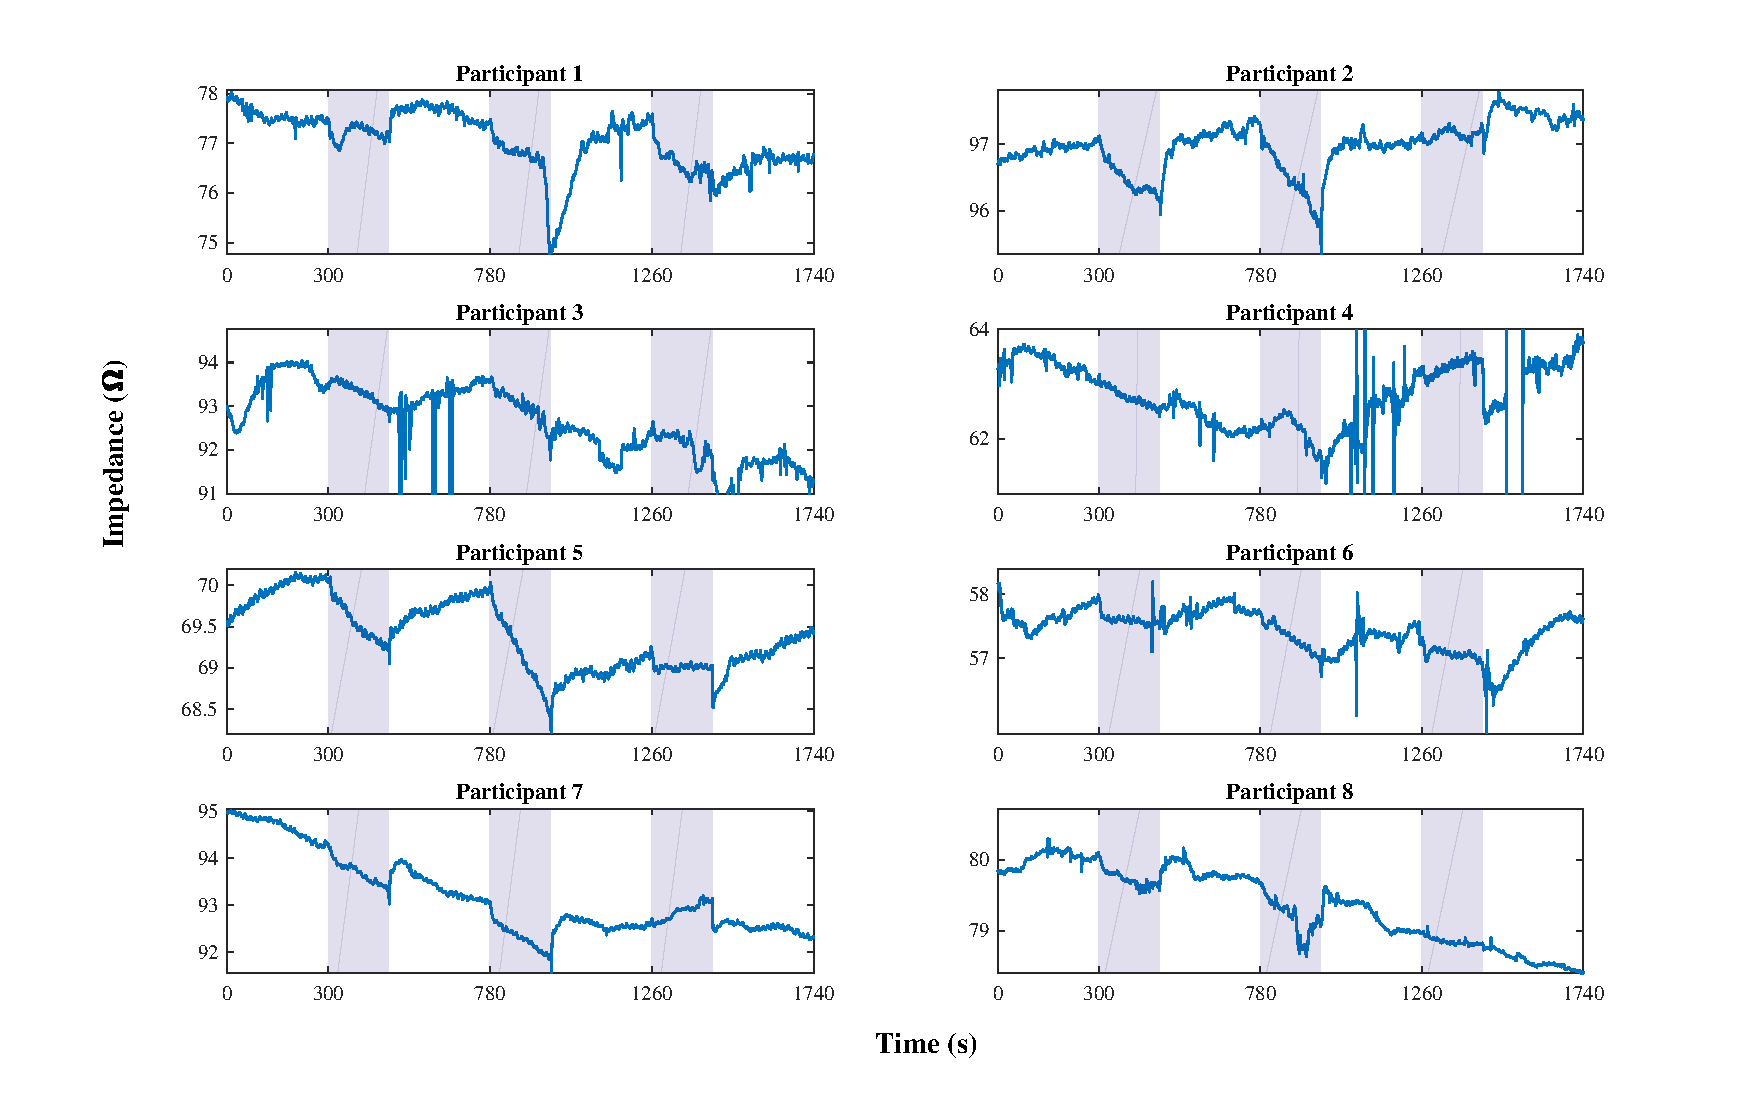
\includegraphics[width=1\textwidth,keepaspectratio,trim={0.75cm 0cm 2cm 2cm},clip]{figure1}    
	\caption[Fequency components of the signals acquired]{Blood flow calculated from venous occlusion plethysmography}
	\label{fig:fft signals}
\end{figure}

\begin{table}[!htbp]
	\caption[Peak frequency calculated obtained form Fast Fourier Transform]{Cardiac frequency obtained from the Fast Fourier Transform for each of the instruments used during the experiment. This peak corresponds to the one with in the hearth cycle in the study (\SI{0.5}{\hertz} < $f_p$ > \SI{1.5}{\hertz})}
	\label{tbl:fft}
	\centering 
	\begin{tabular}{lccccc}
		\toprule
		& \textbf{ECG}
		& \textbf{iPG}
		& \textbf{PPG}
		& \textbf{LDF}
		& \textbf{DU} \\
		& \textbf{$f_p$ [\si{\hertz}]}		
		& \textbf{$f_p$ [\si{\hertz}]}		
		& \textbf{$f_p$ [\si{\hertz}]}
		& \textbf{$f_p$ [\si{\hertz}]}
		& \textbf{$f_p$ [\si{\hertz}]}\\\midrule
	    Participant 1    &     0.967    &     0.952    &     0.949    &     0.897    &     0.949    \\  
		Participant 2    &     0.964    &     0.964    &     0.989    &     0.964    &     0.964    \\  
		Participant 3    &     1.041    &     0.916    &     1.041    &     1.038    &     1.019    \\  
		Participant 4    &     1.425    &     1.437    &     1.422    &     1.321    &     1.425    \\  
		Participant 5    &     0.940    &     0.940    &     0.937    &     0.940    &     0.940    \\  
		Participant 6    &     1.239    &     1.242    &     1.242    &     1.233    &     1.239    \\  
		Participant 7    &     1.163    &     1.163    &     1.163    &     1.163    &     1.163    \\  
		Participant 8    &     1.346    &     1.401    &     1.337    &     1.367    &     N/A    \\  
 
	\bottomrule
	\end{tabular}
\end{table}


%********************************** %Second Section  *************************************
\section{Correlation between iPG AC waveform and Ultrasound Doppler} %Section - 6.2
\label{section correlation 2} 
The Chapter  \ref{chapter results} showed how the waveforms obtained during the experiment changed in amplitude at each occlusive event. By observing the equation \ref{eq:doppler}  from the Doppler ultrasound section can be derived that the velocity ($v$) is directly proportional to the Doppler frequency ($f_D$). The rest of the terms can be assumed as constant. After that, the same rule obeys when the velocity is converted to blood flow. Equally, the blood flow calculated from the iPG device with equation \ref{eq:bf} is a function of $R_B$ which is a directly proportional to the amplitude of the impedance waveform at the point $R_{M5}$ as shown by equation \ref{eq:RB}. In other words, the magnitude of both measurements changes according to the blood flow.

However, the Doppler ultrasound is only focused on arterial flow over the blood vessel under observation. Instead, iPG sees flow changes of both arterial and venous circulation in the volume segment under test. Both devices measure blood flow but in a different way. The Doppler ultrasound requires precision when placing the head of the instrument on the patient's skin. The best signal is obtained when the device is exactly over the blood vessel. Hence, the clarity of the signal depends on the operator skills to maintain a constant angle and always over the artery. During the experiment, this procedure was replicated using laboratory instruments keeping both angle and skin contact constant. Although, using this set-up does not counter rest the participant's arm movement which causes a misaligning of the sensor. As a result, the amplitude of the ultrasound signal is not as steady as one might expect. 

As it was observed in section \ref{section: correlation 1} the AC components of the iPG device is not clean of noise in all the partakers. In fact, participant 2, 5, 6 and 7 showed the best signals to work with. For this reason, the waveforms from these partakers were used when performing the correlation between both instruments. 

Figure \ref{fig:corr FWUS} shows the correlation between both iPG and DU. The data range corresponds to the whole duration of the experiment as includes the changes of blood flow caused by the occlusions. In the plot, the data was discriminated with a different marker point and colour according to every event during the test. As a reminder, odd regions are baselines, and even regions are blockages.  

\begin{figure}[!htpb]
	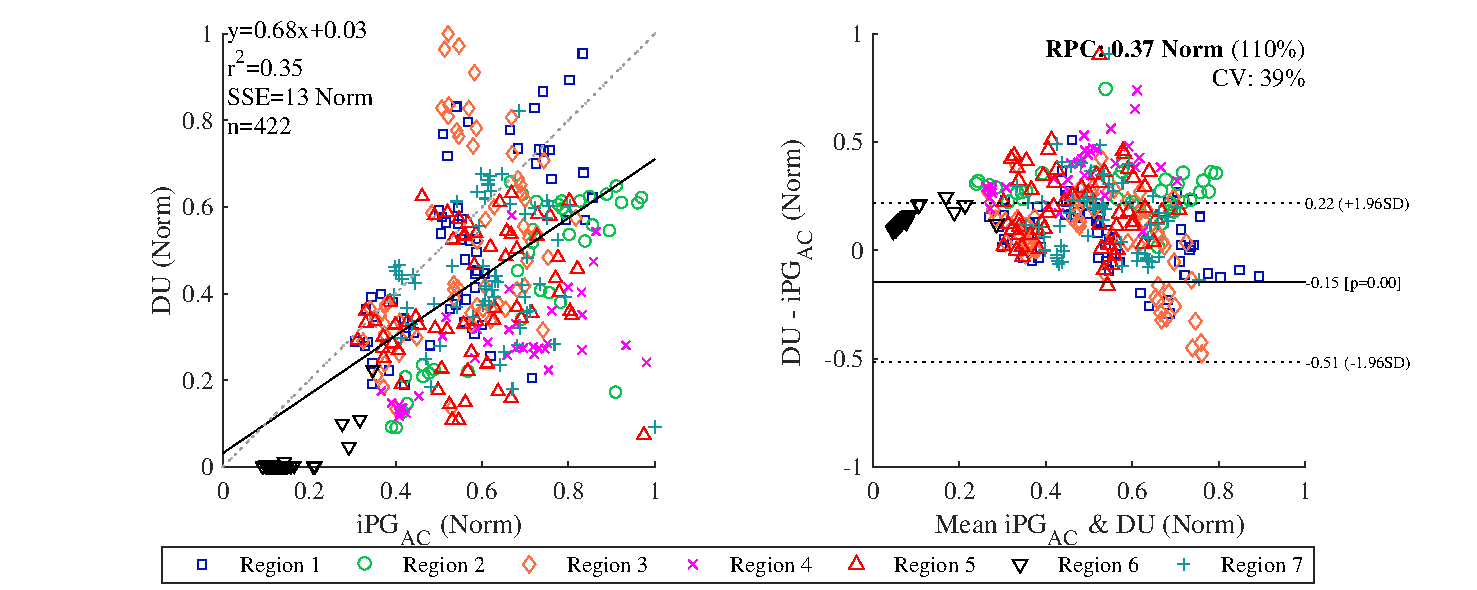
\includegraphics[width=1\textwidth,keepaspectratio]{figure2}    
	\caption[Bland and Altman plot of the relation between Doppler ultrasound and iPG]{Bland and Altman~\cite{bland1986statistical} plot of the relation between Doppler ultrasound and iPG. Data set corresponds to participants 2, 5, 6 and 7.  The data has been normalised comparing the amplitude of both measurements. The different regions has been plotted with various colours and symbols to differentiate every event. The dotted line represents the perfect agreement, the dark line is the linear regression.}
	\label{fig:corr FWUS}
\end{figure}

The data was normalised referenced to the highest peak of the total data set.  Each systolic peak detected from the iPG waveform was used to the find the corresponding Doppler ultrasound systolic peak around the same segment of time. Then the iPG and DU data sets were smoothed by calculating the mean value of every 20 peaks detected in a non-accumulative average.  

The method used to analyse the correlation of both measurements is the method proposed by Bland et al.~\cite{bland1986statistical}. This method allows comparing a traditional technique with a new method. So, it is ideal to compare the measurements between DU and the designed device. This technique is mostly used to compare similar units measurements, for this reason, the data were normalised. Therefore, the comparison will be on the change of magnitude between both modalities.

On the left of the plot can be seen the result of the linear regression between both waveforms. At certain degree the data trend is off the line of equity (dotted line), meaning that there is not a perfect agreement between both methods concerning their amplitudes. In fact, this graph portrays that the linear correlation between both signals with a coefficient correlation  $r^2 = 0.35$ confirming that both signals are related. However, there is not a perfect agreement because of the variability of the reference signal (DU) alongside the y-axes. 

Analysing region by region can be seen how the data points were distributed along the correlation graph. For instance, there seems to be a good distribution of data in both axes in regions 1 and 2. Clearly, both waveforms amplitudes spread quite uniformly. The region 1 appears to be closer to the line of equity than the region 2 when venous occlusion happened. It seems that the magnitude of the DU signal did not change as much as the iPG's ones. Undeniably, the impedance plethysmography device detected changes that the DU could not notice. Which, it is in agreement as the venous occlusion does not alter the arterial flow. 

However, region 3 shows a larger distribution of data points adjacent to y-axes than iPG. Participants movement would have caused this significant variation of the DU amplitude. By reviewing the envelope of the signal on figure \ref{fig:DU_flow} is noticeable that Participant 7 showed the largest waveform amplitudes, this can also be seen in the mean blood flow computed on that same region. In fact, running the data without this participant, the linear regression improves to $r^2 = 0.45$. 

The region 4 displays a similar behaviour as the region 2; there is a good data distribution, but the iPG amplitude changed more than the DU. Nonetheless, there is a greater concentration of data points in the lower region of both axes. This performance would be expected as there is a reduction of arterial blood during this event. The higher data points towards the iPG axes are related to the blood flow rush at the beginning of the occlusion on participant 7, as shown in \ref{fig:blood_flow_plethysmography}.

The region 5 shows a greater distribution of the data adjacent to the iPG axes. On the other hand, there are some data points on the lower part of the DU axes that affect the linear regression in this region. During total occlusion in region 6, there is a better response of the DU device. Here, a significant number of the Doppler's ultrasound data points are set to zero, whereas the data from iPG is mostly distributing among 0 and 0.2. Finally, the Region 7 shows a good distribution adjacent to the line of equity which agrees with some of the other baseline behaviour.

The plot on the right of figure \ref{fig:corr FWUS} shows the precision between the estimated limits of agreement of the whole experiment.  On the y-axes is plotted the mean difference between both measurements and the points of its standard deviation. The differences have normally been distributed in a Gaussian space. Hence \SI{95}{\percent} of the difference should lie between  $\pm$1.96SD). This graph shows that there is a high number of points out of $+$1.96SD. However, it can be noticed that values from regions 2 and 4 are outside the agreement region. Confirming, that when an occlusion occurs there is a different response between iPG and DU.


%********************************** % Third Section  *************************************
\section{Correlation between iPG and PPG}  %Section - 6.3 
\label{section correlation 3}

\begin{figure}[!htpb]
	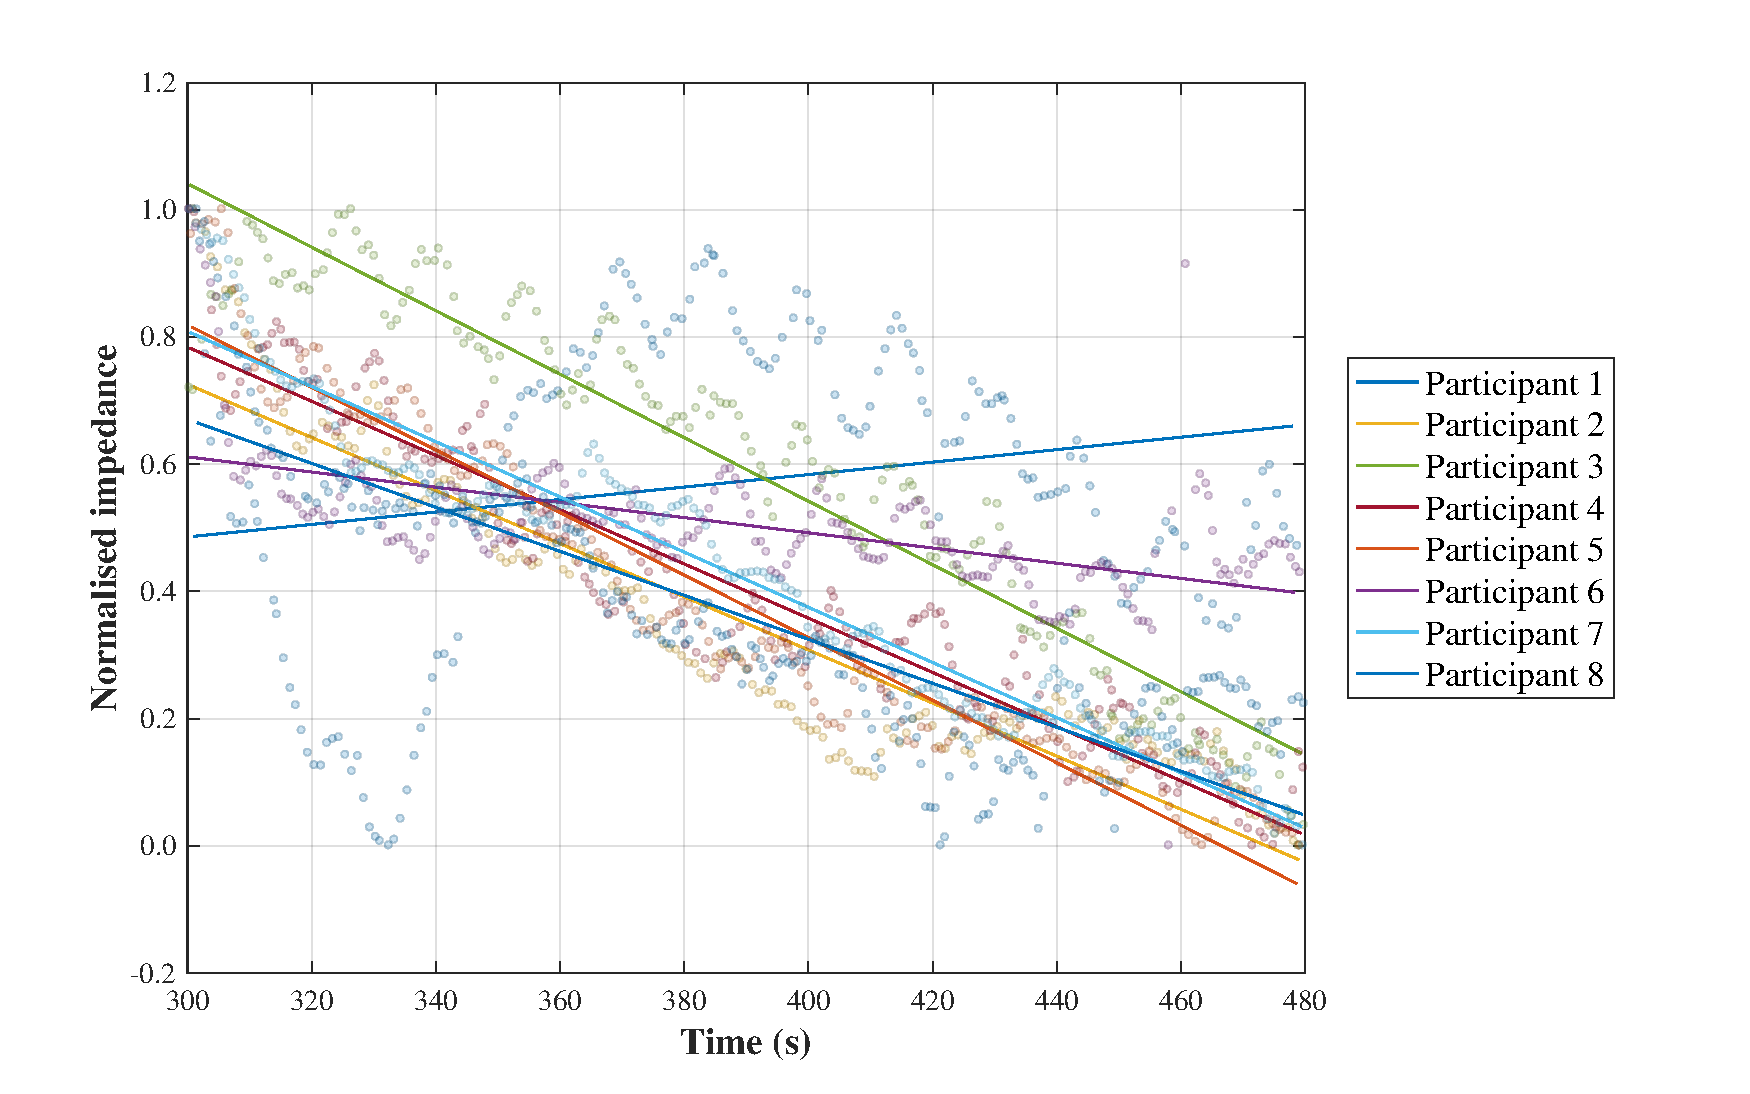
\includegraphics[width=1\textwidth,keepaspectratio]{figure3}    
	\caption[Bland and Altman plot of the relation between PPG and iPG]{Bland and Altman~\cite{bland1986statistical} plot of the relation between PPG and iPG. Data set corresponds to participants 2, 5, 6 and 7. The data has been normalised comparing the amplitude of both measurements. The different regions has been plotted with various colours and symbols to differentiate every event. The dotted line represents the perfect agreement, the dark line is the linear regression.}
	\label{fig:corr RED}
\end{figure}

%********************************** % Third Section  *************************************
\section{Correlation between iPG and LDF}  %Section - 6.4 
\label{section correlation 4}

\begin{figure}[!htpb]
	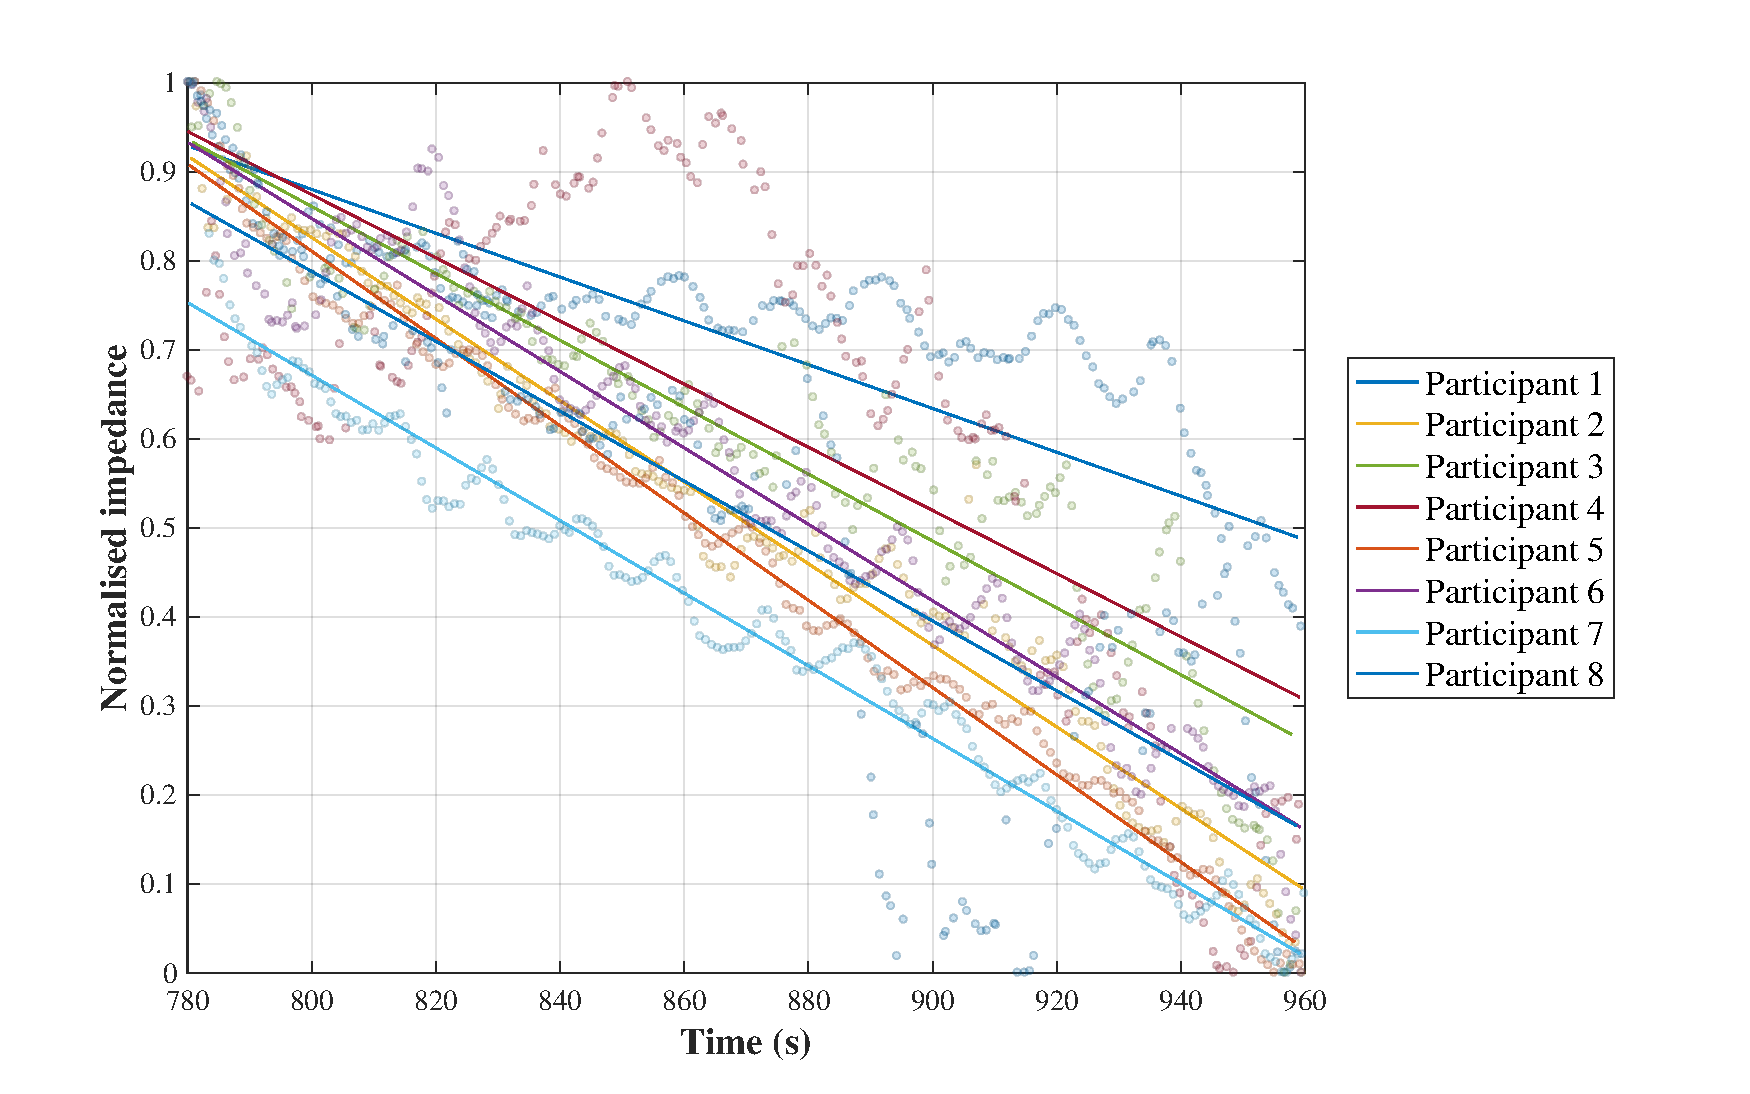
\includegraphics[width=1\textwidth,keepaspectratio]{figure4}    
	\caption[Bland and Altman plot of the relation between LDF and iPG]{Bland and Altman~\cite{bland1986statistical} plot of the relation between LDF and iPG. Data set corresponds to participants 2, 5, 6 and 7. The data has been normalised comparing the amplitude of both measurements. The different regions has been plotted with various colours and symbols to differentiate every event. The dotted line represents the perfect agreement, the dark line is the linear regression.}
	\label{fig:corr LDF}
\end{figure}

